\documentclass[twoside]{article}

% Fonts + Colors ~~~~

\usepackage{lipsum}
\usepackage{fontspec}
\usepackage{dashrule}
\usepackage[export]{adjustbox}
\usepackage[usenames, dvipsnames]{color}
\usepackage{comment}

\definecolor{Gray}{RGB}{120, 120, 120}
\definecolor{LogoRed}{RGB}{153, 0, 0}
\definecolor{LogoTurquoise1}{RGB}{1, 123, 147}
\definecolor{LogoTurquoise2}{RGB}{0, 158, 171}
\definecolor{LogoTurquoise3}{RGB}{0, 186, 187}
\definecolor{BackgroundBlue}{RGB}{247, 254, 255}
\definecolor{LightBlue}{RGB}{230, 247, 255}
\definecolor{LightRed}{RGB}{231, 103, 97}
\definecolor{DarkGray}{RGB}{71, 71, 71}

\begin{comment}
\newfontfamily\Avenir[
    Path= fonts/,
    Extension= .otf,
    UprightFont = *-45Book,
    ItalicFont = *-45BookOblique,
    BoldFont = *-95Black,
]{AvenirLTStd}

\newfontfamily\TradeGothic[
    Path = fonts/,
    Extension = .otf,
    UprightFont = *-No18,
    BoldFont = *-No20Bold,
]{TradeGothicCondensed}

\setmainfont[Ligatures=TeX]{Avenir}
\Avenir\fontsize{9pt}{12pt}\selectfont

\end{comment}

\usepackage[condensed]{roboto}
\usepackage[default,osfigures,scale=0.95]{opensans}
\usepackage[T1]{fontenc}

\fontsize{9pt}{12pt}\selectfont

% Formatting ~~~~

\usepackage{geometry}

\geometry{
    letterpaper,
    top=1.75in,
    bottom=1.75in,
    inner=0.75in,
    outer=0.75in,
    headsep=1in,
    headheight=0.5in,
    footskip=1in,
    % showframe
}

\usepackage[document]{ragged2e}
\parskip=8pt
\parindent=0pt
\linespread{1.2}
\setlength{\columnsep}{0.75cm}

% \usepackage{sectsty}
% \sectionfont{\fontfamily{pag}\selectfont\color{LogoTurquoise1}\vspace{-\parskip}\Large\uppercase}
% \subsectionfont{\color{LogoTurquoise1}\vspace{-\parskip}\mdseries\Large}

\usepackage{titlesec}
\titleformat*{\section}{\fontfamily{pag}\selectfont\color{LogoTurquoise1}\vspace{-\parskip}\bfseries\Large\uppercase}
\titleformat*{\subsection}{\color{LogoTurquoise1}\vspace{-\parskip}\Large}


% Headers + Footers ~~~~

\usepackage{fancyhdr}
\pagestyle{fancy}

\renewcommand{\sectionmark}[1]{\markboth{#1}{}}
\usepackage{fourier-orns}

\fancyhead{} % clear all header fields
\fancyfoot{} % clear all footer fields
\fancyfoot[LE]{\thepage \hspace{0.4cm} \roboto\selectfont\textcolor{LightRed}{\uppercase{Recruiting the Out-of-State University}}}
\fancyfoot[RO]{\roboto\selectfont\textcolor{Gray}{\leftmark} \hspace{0.4cm} \thepage}
\renewcommand{\headrulewidth}{0pt}

\fancypagestyle{tablepage}{  % No Header, Regular Footer
    \fancyhead{}
    \fancyfoot{}
    \renewcommand\headrule{\hrulefill
\raisebox{-2.1pt}[10pt][10pt]{\quad\decofourleft\decotwo\decofourright\quad}\hrulefill}
}

\addtolength{\skip\footins}{10pt}


% Links + Lists ~~~~

\PassOptionsToPackage{hyphens}{url}\usepackage[colorlinks=true, linkcolor=cyan, urlcolor=blue, citecolor=blue, breaklinks=true]{hyperref}
\newcommand{\superscript}[1]{$^{#1}$}

%reference list stuff
\usepackage[natbibapa]{apacite}

%\usepackage[super,numbers]{natbib}

\makeatletter
\renewcommand\@biblabel[1]{\superscript{#1}}
\makeatother

\renewcommand{\refname}{\vspace{-0.65cm}}

\usepackage{enumitem}
\setlist{nosep, itemsep=0pt, parsep=0pt}

\renewcommand{\labelitemi}{\color{LightRed}$\triangleright$}
\renewcommand{\labelitemii}{\color{LogoTurquoise2}$\cdot$}
\renewcommand\labelitemiii{$\circ$}


% Block Formats ~~~~

\usepackage{mdframed}

\newenvironment{quote-block}{  % quote block
    \begin{quote}
    \roboto\selectfont
    \color{LogoTurquoise2}
}
{
    \end{quote}
}

\newenvironment{color-block}[1][Key Points]{  % text block
    \vspace{0.5cm}
    \begin{mdframed}[backgroundcolor=LightBlue, linecolor=LightBlue, userdefinedwidth=\textwidth, leftmargin=0cm, innerleftmargin=1cm, innerrightmargin=2cm, innertopmargin=0.5cm, innerbottommargin=1cm]
    \color{DarkGray}
    \subsection*{\color{LogoTurquoise1}{\Large#1}}
    \vspace{-0.2cm}
}
{
    \end{mdframed}
    \vspace{0.2cm}
}


% Figures ~~~~

\usepackage{graphicx}
\usepackage{caption}
\usepackage[labelformat=simple]{subcaption}

\DeclareCaptionSubType*{figure}
\renewcommand\thesubfigure{}

\DeclareCaptionFont{CaptionFont}{\roboto\selectfont}
\DeclareCaptionFont{LightRed}{\color{LightRed}}

\captionsetup{labelfont={CaptionFont, LightRed}, figurename=FIGURE, tablename=TABLE}

\newcommand{\addFigure}[4][0.2] {  % Add single figure
\begin{figure}[!ht]
    \vspace{0.45cm}
    \centering

    \includegraphics[width=0.45\textwidth, trim={0 0 0 #1cm}, clip]{images/#2}
    \caption{\roboto\selectfont\textcolor{Gray}{\uppercase{#3}}}
    \label{fig:#4}

\end{figure}
}

\usepackage{stfloats}
\newcommand{\addFigureSet}[4] {  % Add 2x2 figure set
\begin{figure*}[#4]
    \vspace{0.45cm}
    \centering

    \begin{subfigure}[b]{.45\linewidth}
      \includegraphics[width=\linewidth, cfbox=Gray 0.4pt]{images/maps/#1_1}
      \caption{1}
    \end{subfigure}\hfill
    \begin{subfigure}[b]{.45\linewidth}
      \includegraphics[width=\linewidth, cfbox=Gray 0.4pt]{images/maps/#1_2}
      \caption{2}
    \end{subfigure}

    \smallskip

    \begin{subfigure}[b]{.45\linewidth}
      \includegraphics[width=\linewidth, cfbox=Gray 0.4pt]{images/maps/#1_3}
      \caption{3}
    \end{subfigure}\hfill
    \begin{subfigure}[b]{.45\linewidth}
      \includegraphics[width=\linewidth, cfbox=Gray 0.4pt]{images/maps/#1_4}
      \caption{4}
    \end{subfigure}

    \caption{\roboto\selectfont\textcolor{Gray}{\uppercase{#2}}}
    \label{fig:#3}

    \ifnum\pdfstrcmp{#4}{b}=0
      \vspace{-1cm}
    \else
      \vspace{0.45cm}
    \fi

\end{figure*}
}

\newcommand{\addSmallMultiples}[3] {  % Add 3x5 figure set
\begin{figure*}[t]
    \vspace{0.45cm}
    \centering

    \includegraphics[width=0.3\textwidth, cfbox=Gray 0.4pt, trim={0 1cm 0 0}, clip]{graphs/199193/#1}\hfill
    \includegraphics[width=0.3\textwidth, cfbox=Gray 0.4pt, trim={0 1cm 0 0}, clip]{graphs/186380/#1}\hfill
    \includegraphics[width=0.3\textwidth, cfbox=Gray 0.4pt, trim={0 1cm 0 0}, clip]{graphs/196097/#1}

    \smallskip

    \includegraphics[width=0.3\textwidth, cfbox=Gray 0.4pt, trim={0 1cm 0 0}, clip]{graphs/100751/#1}\hfill
    \includegraphics[width=0.3\textwidth, cfbox=Gray 0.4pt, trim={0 1cm 0 0}, clip]{graphs/106397/#1}\hfill
    \includegraphics[width=0.3\textwidth, cfbox=Gray 0.4pt, trim={0 1cm 0 0}, clip]{graphs/110635/#1}

    \smallskip

    \includegraphics[width=0.3\textwidth, cfbox=Gray 0.4pt, trim={0 1cm 0 0}, clip]{graphs/110653/#1}\hfill
    \includegraphics[width=0.3\textwidth, cfbox=Gray 0.4pt, trim={0 1cm 0 0}, clip]{graphs/201885/#1}\hfill
    \includegraphics[width=0.3\textwidth, cfbox=Gray 0.4pt, trim={0 1cm 0 0}, clip]{graphs/126614/#1}

    \smallskip

    \includegraphics[width=0.3\textwidth, cfbox=Gray 0.4pt, trim={0 1cm 0 0}, clip]{graphs/139959/#1}\hfill
    \includegraphics[width=0.3\textwidth, cfbox=Gray 0.4pt, trim={0 1cm 0 0}, clip]{graphs/155317/#1}\hfill
    \includegraphics[width=0.3\textwidth, cfbox=Gray 0.4pt, trim={0 1cm 0 0}, clip]{graphs/166629/#1}

    \smallskip

    \includegraphics[width=0.3\textwidth, cfbox=Gray 0.4pt, trim={0 1cm 0 0}, clip]{graphs/181464/#1}\hfill
    \includegraphics[width=0.3\textwidth, cfbox=Gray 0.4pt, trim={0 1cm 0 0}, clip]{graphs/215293/#1}\hfill
    \includegraphics[width=0.3\textwidth, cfbox=Gray 0.4pt, trim={0 1cm 0 0}, clip]{graphs/218663/#1}

    \caption{\roboto\selectfont\textcolor{Gray}{\uppercase{#2}}}
    \label{fig:#3}
\end{figure*}
}


% Tables ~~~~

\usepackage[figuresright]{rotating}
\usepackage{multirow}
\usepackage[table]{xcolor}

\usepackage{etoolbox}
\AfterEndEnvironment{table-env}{\restoregeometry\twocolumn}

\newenvironment{table-env}[3][10]{
  \clearpage
  \newgeometry{top=0.5in, bottom=1in, inner=0.75in, outer=0.75in, footskip=0.25in}
  \begin{sidewaystable}
  \fontsize{8pt}{#1pt}\selectfont
  \ifnum\pdfstrcmp{#2}{x}=-1
    \rotatebox[origin=c]{270}{\begin{minipage}{\textwidth}\caption{\roboto\selectfont\textcolor{Gray}{\uppercase{#2}}}\label{tbl:#3}\end{minipage}}
  \fi
}
{
  \end{sidewaystable}
  \clearpage
}

\newcommand{\addTable}[4][p] {  % Add Table

\begin{table*}[!hb]

    \ifnum\pdfstrcmp{#1}{l}=0
      \begin{sideways}
    \fi

    \centering

    \begingroup
      \fontsize{8pt}{10pt}\selectfont
      \input{tables/#2.tex}
    \endgroup

    \ifnum\pdfstrcmp{#1}{l}=0
      \end{sideways}
    \fi

    \vspace{0.2cm}
    \caption{\roboto\selectfont\textcolor{Gray}{\uppercase{#3}}}
    \label{tbl:#4}

    \vspace{-1cm}

\end{table*}

}


\usepackage{Sweave}
\begin{document}
\sloppy

\Sconcordance{concordance:joyce_report.tex:joyce_report.Rnw:%
1 4 1 1 0 4 1 1 18 486 1}



% Title Page ~~~~

\pagecolor{BackgroundBlue}
\newgeometry{top=0cm, bottom=0cm, left=0cm, right=0cm}
\begin{titlepage}

        \makebox[0pt][l]{%
          \raisebox{-0.49\totalheight}[0pt][0pt]{%
          \scalebox{-1}[1]{
            
\includegraphics[width=9in]{./images/layer.png}}}}%

        \hspace{-0.7cm}
        \makebox[0pt][l]{%
          \raisebox{-1.43\totalheight}[0pt][0pt]{%
            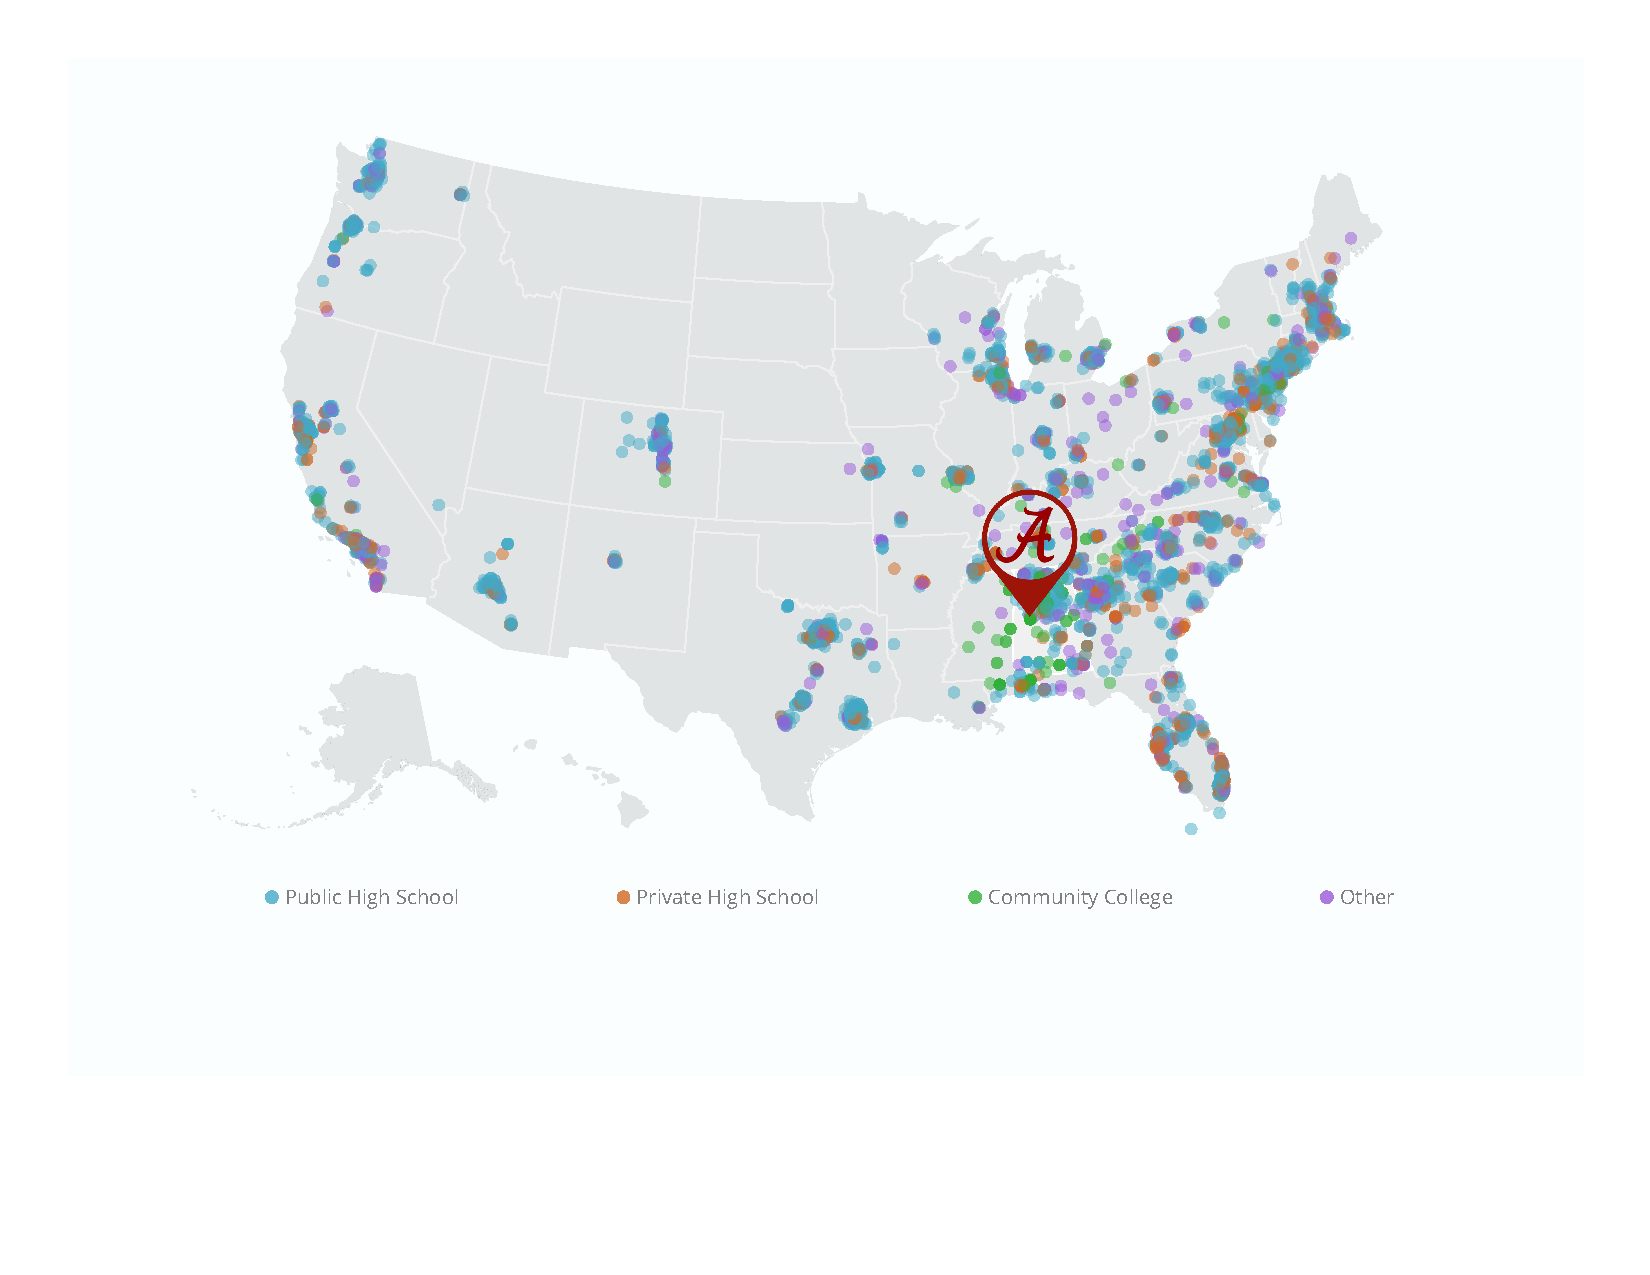
\includegraphics[width=9in, trim={2cm 0 2cm 2cm}, clip]{./images/map_ua.pdf}}}%

        \makebox[0pt][l]{%
          \raisebox{-1.44\totalheight}[0pt][0pt]{%
            
\includegraphics[width=9in]{./images/layer.png}}}%

        \centering\color{DarkGray}\fontsize{30}{60}

        \vspace{0.3cm}
        \hdashrule{0.8\textwidth}{1pt}{1pt} \\

        \vspace{0.8cm}
        \textbf{\color{LogoRed}{RECRUITING}} \\
        \vspace{0.2cm}
        \textbf{\color{LogoRed}{THE OUT-OF-STATE UNIVERSITY}}

        \vspace{0.2cm}
        \Large\textit{\fontfamily{pag}\selectfont Off-campus recruiting by public research universities} \\

        \vspace{0.3cm}
        \hdashrule{0.8\textwidth}{1pt}{1pt} \\

	\vspace{17.1cm}
        \large Crystal Han \\
        Ozan Jaquette \\
        Karina Salazar \\~\\
        %\textit{\color{Gray}{March 2019}}

\end{titlepage}

% Blank Page ~~~~
 
\pagecolor{LightBlue}
\begin{titlepage}
    \color{LightBlue}{x}
\end{titlepage}

% Begin Template ~~~~

\pagecolor{white}
\restoregeometry
\setcounter{page}{1}
\twocolumn

\parskip=14pt
\linespread{1.3}

\section*{Executive Summary\markboth{Executive Summary}{}}  % text inside \markboth{} is displayed in footer

Despite a historical mission of social mobility for meritorious state residents, public research universities increasingly enroll an affluent student body that is unrepresentative of the socioeconomic and racial diversity of the states they serve.  Mainstream policy debates about the causes of access inequality focus on ``deficiencies'' of students and K-12 schools (e.g., the ``achievement gap,'' ``under-matching'').  Public universities positions themselves as remaining committed to access despite state funding cuts and despite student deficiencies, pointing to the adoption of access-oriented policies (e.g., need-based financial aid, outreach programs) as evidence of this commitment. Therefore, this discourse assumes that doubling the number of high-achieving, under-represented students who apply to a university will double their enrollment.  In turn, policy interventions to increase college access focus on changing student behavior rather than university behavior.

An alternative explanation for access inequality is that university enrollment priorities of public research universities are biased against poor students and/or communities of color. Decades of research on organizational behavior finds that internal resource allocation is a reliable indicator of organizational priorities, while policy adoption is often a ceremonial effort to appease external stakeholders, suggesting a ``trust but verify'' approach to university rhetoric about access.  Scholarship on ``enrollment management'' shows that universities are very purposeful about which students they pursue and expend substantial resources crafting their class.  Therefore, knowing which student populations are targeted by university recruiting efforts can yield reliable insights about university enrollment priorities.

%Decades of research on organizational behavior finds that policy adoption is often a ceremonial effort to appease external stakeholders, while internal resource allocation provides a reliable indicator of organizational priorities. These findings suggest a ``trust but verify'' approach to university rhetoric about access
%often represents a ceremonial effort to appease external stakeholders rather than a substantive effort to solve the problem

This report analyzes off-campus recruiting visits (e.g., visit to a local high school) by 15 public research universities as a means of gaining insight about university enrollment priorities. We collected data on recruiting visits by “scraping” data from university admissions websites (e.g., webpages advertising admissions representatives coming to a ``neighborhood near you'') and by issuing public records requests.

\textbf{Findings}. We find a startling degree of socioeconomic and racial bias in university off-campus recruiting patterns.

\textbf{Out-of-state recruiting visits}
\begin{itemize}
    \item Most public research universities prioritize recruiting out-of-state students rather than students from their home state.  X of 15 universities made more out-of-state visits than in-state visits and X of 15 universities made more than twice as many out-of-state visits than in-state visits.
    \item Visits are concentrated in highly affluent communities in major metropolitan areas, ignoring rural communities
    \item All universities were much more likely to visit public high schools in high-income communities than schools in low-income communities, even after controlling for factors associated with making a recruiting visit (e.g., enrollment size, academic achievement, school type)
    %\item Visits to public high schools exhibit dramatic income bias, even after controlling for factors associated with making a recruiting visit (e.g., enrollment size, academic achievement, school type)
    \item Most universities were significantly less likely to visit public high schools with a high percentage of Black, Latinx, and Native American enrollment, even after controlling for factors associated with making a recruiting visit
    %\item For most universities, visits to public high schools exhibit significant racial bias, even after controlling for factors associated with making a recruiting visit
    \item Most universities visit a disproportionate number of out-of-state private high schools
\end{itemize}

\textbf{In-state recruiting}
\begin{itemize}
    \item Even after considering state size and population, "coverage" of in-state public high schools varies dramatically across universities (e.g., University of Nebraska visited X\% of high schools while University of Alabama visited X\%), as does coverage of community colleges
    \item For most universities, visits to public high schools exhibit significant income bias (albeit less than out-of-state visits), even after controlling for factors associated with making a recruiting visit
    \item The presence of racial bias in visits to public high schools differed across universities, with some universities less likely to visit schools with a high share of Black/Latinx/Native students (e.g., University of Alabama) and other universities were more likely to visit schools with a high share of Black/Latinx/Native students (e.g., University of California-Irvine)
\end{itemize}  

\textbf{Overall patterns}
\begin{itemize}
    \item Most universities followed the pattern of limited in-state recruiting and expansive out-of-state recruiting in large metropolitan areas, but the ``regional'' (e.g., Northeast, Midwest, Southeast) focus of out-of-state recruiting differed across universities
    \item Recruiting patterns are clearly tied to state funding. Universities with weak state funding (e.g., University of Alabama, University of South Carolina) focus recruiting efforts out-of-state, make fewer in-state visits, and exhibit socioeconomic and/or racial bias in in-state visits. By contrast, universities with strong state funding (e.g., North Carolina State University, University of California-Irvine) make fewer out-of-state visits, more in-state visits and in-state visits are less likely to exhibit socioeconomic or racial bias
    \item However, universities with similar external environments (e.g., state funding, growth/decline in ``college age'') population, exhibit substantially different recruiting patterns with respect to in-state vs. out-of-state focus, income bias, and racial bias.  GIVE EXAMPLE? Therefore, university enrollment priorities are choices made by leadership rather than mre functions of environmental conditions.
\end{itemize}  


\textbf{Implications and recommendations}. In contrast to rhetoric from universities leaders, our findings suggest that the enrollment priorities of many public research universities are hostile to state residents, poor students, and communities of color.  These enrollment priorities are a function of a broken system of state higher education finance, which incentivizes many public universities to prioritize out-of-state students with mediocre academic achievement from rich, predominantly White communities. This is not a meritocracy.  We suggest recommendations to policymakers, university leaders, and access advocates to reverse this vicious cycle
	\begin{itemize}
		\item \textbf{State policymakers}. State budget cuts to public research universities rationalized on the grounds that universities can generate alternative revenue sources ignore the fact that universities make up for state budget cuts by prioritizing affluent students.  If state policymakers want flagship public universities to prioritize meritorious state residents, they must re-invest in public higher education by growing state appropriations and/or by increasing need-based grant aid, which will increase the purchasing power of poor students.
		\item \textbf{University leaders}.  A growing body of research shows that generous need-based financial aid combined with aggressive outreach dramatically increases the number of high-achieving, low-income students who apply to and attend public research universities. Therefore, access inequality is a function of university will, rather than merely a function of student deficiencies. University leaders serious about access for under-represented studnets must put their money where there mouth is, rather than putting their money where the money is.
		\item \textbf{Access advocates}.  Advocates for access -- those working inside and outside of universities -- can use our research to start a dialogue with university leaders about the disconnect between stated commitments and actual recruiting behavior. Armed with systematic data about university recruiting behavior, access advocates will no longer be deterred by lofty rhetoric or the adoption of opaque programs with unclear resources. Therefore, the data and findings from this report enable access advocates to hold universities accountable for their stated commitments to access and	provide a foundation for an authentic debate about univeristy priorities.

	\end{itemize}




\section*{Introduction\markboth{Introduction}{}}  % text inside \markboth{} is displayed in footer

The University of Alabama-Tuscaloosa exemplifies that transformation from state flagship university to out-of-state flagship.  Resident freshmen increased from 2,028 in 2002-03 to 3,221 in 2008-09 but declined to 2,412 by 2016-17. By contrast, nonresident freshmen increased dramatically from 626 in 2002-03 to 1,895 in 2008-09 and to 5,147 by 2016-17.  This period was also witnessed the erosion of state appropriations, which had increased from  \$165 million in 2002-03 to \$227 million in 2007-08, but declined sharply to \$149 million by 2010-11 following the Great Recession, increasing only modestly to \$153 million by 2015-16 (2018 CPI).  By contrast, driving by nonresident enrollment growth, net tuition revenue increased dramatically, from \$102 million in 2002-03 to \$220 million by 2007-08 to \$492 million by 2015-16 [UPDATE NUMBERS/YEARS].

Nonresident enrollment growth at the University of Alabama also coincided with declining socioeconomic and racial diversity.  The percent of full-time freshman receiving Pell Grants declined from 21.2\% in 2010-11 to 17.1\% in 2016-17.  Additionally, while the percent of 18-24 year-olds in Alabama who identify as Black increased from 31.4\% in 2010-11 to 32.7\% in 2016-17 [GET NEW YEAR OF DATA?], the percent of full-time freshman at the University of Alabama who identify as Black declined from 11.9\%  in 2010-11 to 7.5\% in 2017-18.

While most research on college access focuses on student behavior, the transformation of student composition at the University of Alabama did not result from sudden, unexpected shifts in student demand. Rather, the University developed arguably the most sophisticated and extensive approach to student recruiting in public higher education.  Utilizing the ``data science'' expertise of enrollment management consulting firms, the university identifies desirable ``prospects'' and plies these prospects with a targeted cocktail of emails, brochures, paid advertising (e.g., pay-per-click ads from Google), off-campus recruiting visits to ``feeder'' high schools, and a savvy social media campaign. 

%This report focuses on off-campus recruiting visits (e.g., visits to local high schools, community colleges, hotel receptions). 
Figure X provides simple descriptive statistics about off-campus recruiting visits (e.g., visits to local high schools, community colleges, hotel receptions) by the University of Alabama in the 2017 calendar year [REVISE PARAGRAPH IN RELATION TO FIGURE].  Admissions representatives made 4,261 off-campus recruiting visits.  However, only 382 of these visits occurred in Alabama.  Further, the University visited only 32\% of Alabama public high schools. These in-state public high school visits were concentrated relatively, affluent, predominantly White communities, largely avoiding high schools in Alabama's ``Black Belt,'' which enroll the largest concentration of African American Students.  However, these in-state recruiting efforts were dwarfed by the 3,879 out-of-state recruiting visits, which spanned metropolitan areas across the U.S. The University made 2,252 visits to out-of-state public high schools. These visits focused on schools in affluent communities, with visited schools having a much higher percent of White students than non-visited schools.  Incredibly, the University made 914 visits to out-of-state private high schools, more than double the total number of in-state recruiting visits.
%WHAT SHOULD SMALL MULTIPLE FIGURE INCLUDE
	% TENTATIVE CHOICE OF SMALL MULTIPLES TO SHOW
	  % timeline of events with different colored lines for event type [would work for flow of paragraph showing the mad rus of "travel season"]
	  % number of events by event-type and in-state vs. out-of-state
	  % median household income of zip codes in visited vs. non-visited public HS by in-state vs. out-of-state
	  % map of alabama, with pins for visted vs. non-visited schools [add backdrop of racial composition?]
	    % this would convey race story nicely; complete ignoring of "black belt"
	% PROBABLY
	  % timeline of events 
	% MAYBE
	  %Map of US
	  %timeline of visits
	  %;number of public HS vs. private HS visits compared to number if visits were random

The University of Alabama represents an extreme case of a transformation occurring at many, but not all, public research universities across the nation.  Public research universities were founded to provide upward mobility for high-achieving state residents \citep{RN2269} and designated the unique responsibility of preparing the the future professional, business, and civic leaders of the state.  Quoting 19th Century University of Michigan President James Angell, these institutions provided ``an uncommon education for the common man'' \citep[as cited in][p. 279]{RN3608} who could not afford tuition at elite private institutions.  Unfortunately, public research universities increasingly an enroll an affluent student body that is unrepresentative of the socioeconomic and racial diversity of the states they serve \citep{RN3685,RN4247}. High-achieving, low-income students in many states are often funneled to community colleges, which dramatically lower the probability of obtaining a BA \citep{RN2261}. By contrast, many public research universities have dramatically increased nonresident enrollment \citep{RN3753} and have adopted financial aid policies that specifically target non-resident students with modest academic achievement \citep{RN1469,RN3762,RN4032,RN4409}. These trends raise concerns that public research universities have transformed from ``engine[s] of social mobility'' \citep[][p. 3]{RN1149} to ``engines of inequality.''

Contemporary policy debates about racial and socioeconomic inequality in college access tend to focus on the ``achievement gap'' and on ``undermatching,'' the idea that high-achieving, low-income students fail to apply to good colleges because they have bad guidance at home and at school \citep{RN4016}.  These explanations focus on ``deficiencies'' of students and K-12 schools. As such, policy interventions to increase college access mostly focus on student academic achievement and decision-making \citep{RN4351}. Policy debates also highlight affordability is an important barrier to access. In recent decades, particularly following the Great Recession of 2008, states disinvested in public universities, and these state budget cuts have been associated with steep rises in tuition price. 

Public research universities position themselves as progressive actors that remain committed to the access mission despite state funding cuts and despite the deficiencies of students and K-12 schools. Universities point to the adoption of policies such as holistic admissions, need-based financial aid, and outreach/pipeline programs as evidence of their commitment to access \citep{RN4017}.  However, decades of research on organizational behavior shows that formal policy adoption (e.g., outreach, financial aid programs) is often a symbolic effort to appease external stakeholders rather than a substantive effort to solve the problem \citep{RN2436}.

Recent trends in enrollment and public funding suggest an alternative explanation for growing racial and socioeconomic inequality in access to public  research universities: university enrollment priorities privilege affluent students and are biased against low-income students and communities of color. Drawing from scholarship on organizational behavior \citep[e.g., ][]{RN513,RN531,RN1714}, we argue that knowing which student populations are actually targeted by university recruiting efforts is a more credible indicator of enrollment priorities than university rhetoric or policy adoption. In turn, scholarship that uses recruiting behavior as an indicator of enrollment priorities has important policy implications; if university enrollment priorities -- the ``supply side'' of higher education -- are biased against low-income students and communities of color, then policy solutions that focus solely on students and K-12 schools -- the ``demand side'' -- will fail to overcome access inequality. 
%If the enrollment priorities of public universities are biased against low-income students and communities of color, then policy solutions that focus solely on students and K-12 schools will fail to overcome access inequality.
%Unfortunately, research on recruiting is rare because data on university recruiting behavior are difficult to obtain. 

%This report on off-campus recruiting visits by public research universities represents the first systematic, quantitative analysis of university recruiting behavior. 
Unfortunately, research on recruiting is rare because data on university recruiting behavior are difficult to obtain.  This report represents the first systematic, quantitative analysis of university recruiting behavior. Specifically, we investigate off-campus recruiting visits by 15 public research universities.  We collected data on off-campus recruiting visits by ``scraping'' the ``travel schedules'' of university admissions officers from university admissions websites (e.g., web-pages advertising admissions representatives coming to a ``neighborhood near you'') and also by issuing public records requests to public universities.  We merged recruiting visit data to secondary data on high schools, community colleges, and communities in order to investigate the characteristics of schools and communities that receive visits.  

The report is organized as follows. First, we provide an overview of the ``enrollment management'' industry and situate off-campus recruiting within the broader set of recruiting interventions employed by universities.  Next, we describe research methodology and present research findings.  The majority of public universities in our sample made far more out-of-state recruiting visits than in-state recruiting visits.  These out-of-state recruiting visits were concentrated in affluent, predominantly White public schools and private schools.  The in-state recruiting visits of many universities also revealed socioeconomic and racial bias, albeit less dramatically than out-of-state visits.  However, a handful of universities -- notably those with stronger state funding -- focused their recruiting efforts on in-state schools and communities and did not exhibit racial or socioeconomic biases.  

Finally, we discuss implications for policymakers and university leaders, with the goal of reversing the vicious cycle of states disinvesting in public universities and public universities disinvesting in the state.  State policymakers often rationalize funding cuts to public research universities on the grounds that these organizations can generate their own revenue sources [CITE].  Policymakers concerned about access must understand that state funding cuts incentivize public research universities to prioritize affluent, out-of-state students. 

Collecting concrete data on university recruiting behaviors also has important implications for university leaders. University leaders can no longer trumpet a commitment to access while simultaneously focusing recruiting efforts on affluent prospects because we are releasing these data to the public. Armed with these data, internal and external constituents committed to access will not be placated by lofty rhetoric and ceremonial action.  Therefore, the time is now for leaders of public research universities to resurrect the historic role as the state's preeminent engine of opportunity and social mobility.


\section*{The Enrollment Management Industry\markboth{The Enrollment Management Industry}{}}  % text inside \markboth{} is displayed in footer

%[TRANSITION PARAGRAPH; TOO LONG?] State budget cuts to public research universities are often rationalized on the grounds that organizations can generate their own revenue sources [CITE]. This is often true and tuition revenue is the biggest money-maker for most universities. What policymakers have ignored is that public universities respond to state disinvestment by shifting ``enrollment management'' operations towards the recruitment of students that generate substantial tuition revenue and often by focusing on the pursuit of rankings prestige at the expense of access for state residents.  Therefore, an understanding of how the enrollment management industry works is the first step to understanding the link between state funding policy and university enrollment behaviors.
%Understanding how the enrollment management industry works is the first step to understanding the link between state funding policy and university enrollment behaviors.  

Understanding the relationship between university enrollment behaviors and access inequality requires a basic understanding of the enrollment management industry.  Enrollment management (EM) is a profession that integrates techniques from marketing and economics in order to ``influence the characteristics and the size of enrolled student bodies'' \citep[p.~xiv]{RN2771}.  EM is also a university administrative structure (e.g., "The Office of Enrollment Management") that coordinates the activities of admissions, financial aid, and marketing and recruiting. 

The broader enrollment management industry consists of professionals working within universities (e.g., vice president for enrollment management, admissions counselors), the associations EM professionals belong to (e.g., National Association for College Admission Counseling), and the marketing and EM consultancies universities hire (e.g., Hobsons, Ruffalo Noel Levitz).
%for advice about which prospects to recruit, how to identify those prospects, and how to recruit them.

\subsection*{The enrollment funnel}

Figure~\ref{fig:emfunnel} depicts the ``enrollment funnel,'' a conceptual tool the EM industry uses to describe stages in student recruitment in order to inform targeted recruiting interventions.  While scholarship and policy debate about college access focuses on the final stages of the enrollment funnel -- which applicants are admitted \citep[e.g., ][]{RN3536} and financial aid ``leveraging'' to convert admits to enrollees \citep[e.g., ][]{RN1948} -- the EM industry expends substantial resources on earlier stages of the funnel.  ``Prospects'' are ``all the potential students you would want to attract to your institution'' \citep{RN4322}. ``Inquiries'' are prospects that contact the university; these include inquiries who who respond to initial solicitation by the universities (e.g., email, brochure) and inquiries who reach out on their own (e.g., sending SAT/ACT scores to the university, completing a form on the university admissions website).  Most universities hire EM consulting firms, which utilize sophisticated, data-intensive methodologies, to help universities identify prospects, solicit inquiries, convert prospects and inquiries into applicants, etc. For example, from 2010 to XXXX the University of Alabama paid \$2.7 million to the EM consulting firm Hobsons \citep{RN4035}[CRYSTAL UPDATE NUMBERS/YEARS].

%Most universities hire EM consulting firms, which utilize sophisticated, data-intensive methodologies, to make recommendations about which prospects to prioritize, how to identify those prospects, how to solicit inquiries, and how to convert converting prospects and inquiries into applicants, etc.

% Params: width (default: 0.75\textwidth), filename in the images/ folder, caption, fig reference (e.g., ~\ref{fig:funnel})
\addFigure[0.55]{funnel_alt.png}{The Enrollment Funnel.}{emfunnel}


%Most universities hire EM consulting firms -- which integrate university data (e.g., prospects, applicants, and enrollees from previous years) with their own micro data on schools and communities -- to make recommendations about interventions at each stage of the enrollment funnel (e.g., identifying prospects, soliciting inquiries, converting prospects/inquiries into applicants). 


Universities identify prospects primarily by purchasing ``student lists'' from College Board and ACT. From 2010 to XXXX, the University of Alabama paid \$1.2 million to College Board and XXXX to ACT \citep{RN4035} [CRYSTAL UPDATE NUMBERS/YEARS].  \cite{RN4314} found that the median public university purchased 64,000 names. Student lists contain contact details and background information (demographic, socioeconomic, and academic) about individual prospects. Universities control which prospects are included in a list by selecting on criteria such as zip code, race, academic achievement.  

Once identified, prospects are plied with recruiting interventions aimed at soliciting inquiries and applications \citep{RN4323}. Non face-to-face interventions include email, brochures, and text messages.  Face-to-face interventions include on-campus visits and off-campus visits. Additionally, universities utilize paid advertising (e.g., pay-per-click ads from Google, cookie-driven ads targeting prospects who visit your website) and social media (e.g., Twitter, Instagram, YouTube) as a means of generating inquiries and creating positive ``buzz'' amongst prospects \citep{RN4134}. Given the the rise in ``stealth applicants'' who do not inquire before applying \citep{RN4411}, social media enables universities to tell their story to prospects who do not want to be contacted.

Given the focus of this report, what is the role of off-campus visits in student recruitment? In the admissions world, ``travel season'' refers to the mad dash between Labor Day and Thanksgiving when admissions officers host hotel receptions, college fairs, and visit high schools across the country \citep{RN3519}. Research by both EM consulting firms and by scholars describe off-campus recruiting as a means of simultaneously identifying prospects and connecting with prospects already being targeted through mail/email \citep[e.g., ][]{RN4323,RN4315,RN3519}. With respect to efficacy, \cite{RN4402} found that off-campus visits were the second highest source of inquiries (after student list purchases) for the median public university, accounting for 19.0\% of inquiries. Off-campus visits were also the third highest source of enrollees (after stealth applicants and on-campus visits), accounting for 16\% of enrollees \citep{RN4402}.
%across the country with the goal of soliciting applications


Additionally, research finds that high school visits are instrumental for mainitaining warm relationships with guidance counselors at feeder schools.  \cite{RN3519} worked as a regional admissions recruiter for a selective liberal arts college as part of his broader ethnography on college admissions.  Relationships with counselors were essential because ``The College's reputation and the quality of its applicant pool are dependent upon its connections with high schools nationwide'' \citep[p.~53]{RN3519}. Echoing these findings, \cite{RN4402} found that face-to-face meetings were the most effective means of engaging counselors.  \cite{RN3519} found that The College visited the same schools year after year because successful recruiting depends on long-term relationships with high schools. Further, The College tended to visit affluent schools, and private schools in particular, because these schools enroll high-achieving students who can afford tuition and because these schools have the resources and motivation to host a successful visit \citep{RN3519}.  

%VERSION 1
%Additionally, ethnographic research by \cite{RN3519} -- he worked as regional admissions recruiter for a selective liberal arts college -- found that high school visits enabled the College to maintain warm relationships with high school guidance counselors at feeder schools.  Echoing these findings, \cite{RN4402} found that face-to-face meetings were the most effective means of engaging counselors. \cite{RN3519} states that relationships with counselors were essential because ``the College's reputation and the quality of its applicant pool are dependent upon its connections with high schools nationwide'' \citep[p.~53]{RN3519}.  The College visited the same schools year after year because successful recruiting depends on long-term relationships with high schools. The College tended to visit affluent schools, and private schools in particular, because these schools enroll high-achieving students who can afford tuition and because these schools have the resources and motivation to host a successful visit.  

\cite{RN4324} analyzed high school visits from the student perspective. High school visits influenced where students applied and where they enrolled. The strength of this finding was modest for affluent students with college educated parents, who tended to be more concerned about college prestige and less influenced by overtures from colleges. However, this finding was particularly strong for first-generation students and under-represented students of color.  These students often felt that ``school counselors had low expectations for them and were too quick to suggest that they attend community college'' (p. XX) and were drawn to colleges that ``made them feel wanted'' by taking the time to visit.  Therefore, while \cite{RN4324} shows that college choice for under-served student populations often hinges on which colleges and universities take the time to visit, prior research has not systematically investigated which high schools receive visits by which colleges and universities.
%COMMENT 2/11/2019; THIS PARAGRAPH, PARTICULARLY SECOND HALF COULD BE MORE EFFICIENT; FIND WAYS TO REDUCE REDUNDANCY

\subsection*{Enrollment goals and recruiting behavior}

While the EM industry provides tools for identifying and targeting prospects at each stage of the enrollment funnel, university enrollment priorities dictate which prospects universities actually pursue.  The ``iron triangle'' of enrollment management states that universities pursue the broad enrollment goals of academic profile, revenue, and access \citep{RN2772}. ``Academic profile'' refers to enrolling high-achieving students -- particularly with respect to standardized test scores -- who help the university move up the rankings. ``Revenue'' refers to students who generate high net tuition revenue.  For public universities, the ``access'' goal refers to access for state residents, first-generation students, low-income students, and students of color from historically under-represented racial/ethnic groups. Because resources are scarce, the imagery of the iron triangle suggests that pursuing one goal involves trade-offs with other goals: ``most enrollment management policies...do not advance all three objectives; instead they lead to gains in some areas and declines in others'' \citep[p.~221]{RN2772}. Enrollment managers view these trade-offs as an inevitable consequence of organizational enrollment priorities, thereby motivating the question, ``What are the enrollment priorities of public universities?''

Drawing from theories of organizational behavior, we argue that university recruiting behavior is a good indicator of enrollment priorities.  Neo-institutional theory argues that organizations face pressure to publicly adopt goals demanded constituencies in the external environment (e.g., move up in the rankings, increase socioeconomic and racial diversity) \citep{RN513,RN527}. However, organizations have scarce resources and cannot easily pursue goals that conflict with one another.  Rather than publicly rejecting a goal demanded by the external environment, organizations resolve conflicts between stated goals by substantively adopting some goals and symbolically adopting others.  Under substantive adoption, organizations allocate substantial resources towards achieving the goal.  Under symbolic adoption, organizations adopt policies and rhetoric that signal commitment to the goal, but do not allocate substantial resources to achieving the goal.  This perspective on organizational priorities is stated succinctly by the Joe Biden quote, ``don’t tell me what you value. Show me your budget and I’ll tell you what you value'' [CITE].

Off-campus recruiting visits by university admissions staff represent a substantial allocation of resources (e.g., staff salary and benefits, travel costs).  Therefore, we argue that comparing the characteristics of schools and communities that receive recruiting visits to those that do not can yield insights about university enrollment priorities.  By contrast, speeches and policy adoption (e.g., holistic admissions, ``outreach'' programs) \citep[e.g., ][]{RN4017} show which goals are publicly adopted, but do not indicate which goals have been adopted substantively versus symbolically.

\section*{Project overview\markboth{Project overview}{}}

This report presents descriptive results from a broader project that collects data on off-campus recruiting by colleges and universities. Many universities advertise off-campus recruiting events on their admissions websites (e.g. "coming to your area" links).  We used ``web-scraping'' to collect data on recruiting events.  We ``scraped'' web-pages containing recruiting event data once per week from 1/1/2017 to 12/31/2017, thereby capturing recruitment of spring juniors and fall seniors. Here, we provide a broad overview of data collection, data processing, and analysis sample. Appendix X provides additional technical detail on XXXX TOPICS [CRYSTAL/KARINA]

The data collection sample for the broader project was drawn from the population of public research-extensive universities (2000 Carnegie Classification). Out of all public research-extensive universities (N=102), the project collected data for those that posted off-campus recruiting events on their admissions websites (N=40). We also collected recruiting visit data from selective private research  universities and from selective private liberal arts colleges.\footnote{CYRSTAL OR KARINA - ADD BRIEF FOOTNOTE TEXT ABOUT WHICH ORGS WE COLLECTED DATA FROM} For each university in the data collection sample, we investigated the entire university website, searching for URLs that contained data on off-campus recruiting events. This process was conducted independently by two members of the research team to avoid missing any relevant URLs. Our programs also scraped data about participation in national college fairs from the National Association for College Admission Counseling (NACAC) website. We also collected data about participation in "group travel tours" from websites advertising joint recruiting events by multiple universities (e.g. Peach State Tour by Georgia State University, Georgia Tech, and The University of Georgia). Since URLs containing data on off-campus recruiting events often change (e.g., a university creates a new URL or changes the formatting of an existing URL),  we completed this investigation process for each university every two months and data collection scripts were updated accordingly.

\subsection*{Defining off-campus recruiting}

We categorized off-campus recruiting events based on event \textit{type}, \textit{host}, and \textit{location}. Event type includes college fairs (in which multiple colleges attend), day-time high school visits, group travel visits, formal admissions interviews, admitted student events, and committed student events. Event hosts include paid staff, paid consultants (e.g. a regional recruiter contracted by the university), alumni, and current students. Event locations include high schools, community colleges, hotels, conference/convention centers, and other public places (e.g., cafes).  

For the purpose of our research, we define off-campus recruiting events as those that focused on soliciting undergraduate admissions applications and were hosted by paid personnel or consultants at any off-campus location. This definition excludes admitted and committed student events, but includes guidance counselor events. Additionally, we excluded formal one-on-one formal interviews because these events focus on determining admissions eligibility of a particular prospect; they are not events that focus on soliciting applications from many prespective students. We excluded events hosted by alumni or student volunteers because theories of organizational behavior suggest that the activities of paid staff are better indicators of organizational priorities than activities allocated to volunteers \citep{RN531}.
%ADD FOOTNOTE? ^[Or, event may be a virtual event (e.g., webinar, video call) with a target audience at a specific off-campus location (e.g., students from a particular high school)]

\subsection*{Analysis sample}

The analysis sample for this manuscript consists of 15 public research universities. These cases were selected from the larger project sample and selected based on "completeness" of recruiting event data posted on admissions websites.  Based on prior research [e.g. CITE] and conversations with admissions professionals, nearly all colleges and universities convene three broad types of off-campus recruiting events: (1) receptions/college fairs at hotels and convention centers; (2) evening college fairs at local high schools; and (3) day-time visits at local high schools. However, some institutions we collected data from did not post all three types of recruiting events. Of the 40 public research universities we collected data on, these 15 universities posted all three broad types of off-campus recruiting events on their website. 

TABLE X [CRYSTAL ADD] shows how the 15 universities in our sample compare to the population of public research universities. [ADD ONE OR TWO SENTENCES ABOUT SIMILARITIES/DIFFERENCES BETWEEN OUR SAMPLE AND POPULATION]

\subsection*{Data processing and data quality}

We took a multi-step approach to processing information scraped from admissions webpages. First, automated Python scripts scrape all text from admission webpages, storing the information as HTML text in a Structured Query Language (SQL) database on a remote server. Separate scripts parse the HTML text into tabular data (e.g., columns for event date, event time, school name, address). Third, we "geocode" recruiting events, converting limited location information (e.g., school name, city, state) into geographic coordinates. Geocoding scripts take location information, query the Google Maps Application Program Interface (API), and return more detailed geographic information for each event (e.g., latitude and longitude coordinates, county, city, state, full street address, zip code).

We conducted two additional data quality checks. First, we manually checked each scraped recruiting event, ensuring that event "type" (e.g., public high school visit) was correctly categorized and that each event was merged to the correct secondary data source (e.g., the correct NCES school ID). 

[CRYSTAL/KARINA UPDATE THIS PARAGRAPH] Second, we checked the completeness of web-scraped data by issuing public records requests for the list of all off-campus recruiting events and then comparing the two data sources. Specifically, we issued public records requests to X universities. We did not issue requests to XXXX and XXX universities because statutes in these states only permits public records requests from state residents. We received data from XXX universities. XXX universities refused or have not sent us data at the time of this report. For universities that sent us data, we used ``requested'' data rather than ``scraped'' data for the analyses below. Broad patterns were similar across requested data versus scraped data and results based on scraped data are available upon request. [SAY THAT REQUESTED DATA WENT THROUGH MANUAL CHECKS TOO?]



\section*{Results\markboth{Results}{}}

\subsection*{University of Georgia}
\lipsum[4]
% Params: [negative spacing if figure placed at bottom of page], univ_id (which is also the name of the folder inside images/ folder, where the images are located), caption, fig reference, top or bottom of page
\addFigureSet[-1]{139959}{University of Georgia result set.}{uga}{b}
\lipsum[5]

\subsection*{University of California, Berkeley}
\lipsum[4]
\addFigureSet{110635}{UC Berkeley result set.}{ucberkeley}{t}
\lipsum[4]

\subsection*{University of Pittsburgh}
\lipsum[4]
\addFigureSet[-1]{215293}{University of Pittsburgh result set.}{upitt}{b}
\lipsum[5]

\subsection*{Stony Brook}
\lipsum[4]
\addFigureSet{196097}{Stony Brook result set.}{stonybrook}{t}
\lipsum[5]

\section*{Discussion and Implications for Policy and Practice\markboth{Discussion}{}}

\subsection*{Summary and Discussion}

This study investigated off-campus recruiting visits by public research universities, which we argue are indicators of university enrollment priorities.  The majority of universities in our sample made more than twice as many out-of-state recruiting visits than in-state recruiting visits.  These out-of-state visits focused primarily on public schools in affluent, predominantly White communities and with a disproportionate focus on predominantly White private schools.  

%University recruiting behavior is an indicator of enrollment priorities [CUT THIS SENTENCE AND MOVE BELOW?].  This study suggests that the recruiting behavior and enrollment priorities of many public research universities biased against state residents, low-income communities, and [TO A LESSER EXTENT?] communities of color.  
Our data indicate that most universities did not visit the majority of public high schools in their home state. This finding is not an indictment; universities in large, populous states with formalized statewide higher education systems (e.g., the State University of New York) cannot be expected to visit every high school. Nevertheless, some universities covered their home state more thoroughly and more equitably than others.  For example, The University of Nebraska-Lincoln visited most public high schools in Nebraska. SUNY-Stony Brook visited most public high schools in its ``home'' jurisdiction of Long Island. Both NC State and UC-Irvine made more in-state recruiting visits than out-of-state visits and these in-state visits did not exhibit socioeconomic or racial bias.  

By contrast, many universities that focused recruiting efforts on out-of-state schools did a poor job of covering their home state. Some state flagships visited a small proportion of public high schools despite being in less populous states with relatively few public high schools (e.g., University of Alabama, University of Kansas, University of Georgia).  Other state flagships showed pronounced socioeconomic and racial bias in in-state recruiting visits (e.g., UC-Berkeley, OTHER).


To sumarize, several universities -- notably those that receive stronger state funding -- made substantial efforts to cover their home state in an equitable way, but the majority of universities prioritized visits to affluent out-of-state communities and showed bias towards low-income communities and/or communities of color.  In turn, these recruiting patterns suggest that the enrollment priorities of many public research universities are socioeconomically and/or racially biased.  We identify two negative consequences of biased recruiting behaviors and enrollment priorities: first, effects on the academic and social campus culture experienced by enrolled students; and, second, effects on enrollment opportunities at public research universities for under-represented student populations.

 Why should society care about the recruiting behavior and enrollment priorities of public research universities? 
 
%We argue that recruiting behavior is an indicator of enrollment priorities. Therefore, the findings of biases in recruiting patterns suggest biases in enrollment priorities at many public reseearch universities.

\textbf{\textit{Effects on campus culture}}.  Nationally, nonresident students tend to be more affluent and are less likely to be Black or Latinx than resident students \citep{RN3685}. Further, growth in nonresident students is associated with declines in the share of Pell recipients and under-represented minority students at public research universities \citep{RN3685}.  Our research suggests that nonresident enrollment growth is associated with declines in socioeconomic and racial diversity because public research universities are explicitly concentrating visits on affluent, predominantly White out-of-state communities.  In turn, these shifts in student composition have important consequences on enrolled students.  An extensive literature shows that low socioeconomic and racial diversity negatively affects that academic and social experiences of poor students and students of color \citep[e.g., ][]{RN3205,RN3193,RN3639,RN3185} and negatively affects learning outcomes for \textit{all} students \citep[e.g., ][]{RN3026,RN2576,RN3153,RN3174}.

While a handful of internationally prestigious public flagship universities (e.g., UC-Berkeley, University of Michigan) enjoy strong demand from high-achieving out-of-state students, less prestigious public flagship universities (e.g., University of South Carolina, University of Alabama) are more likely to compete for out-of-state prospects who could not gain admission to flagship public universities in their home state.  Indeed, many less-prestigious public flagship universities adopted institutional ``merit'' aid programs that target out-of-state prospects who lack the academic achievement necessary for admission to their own state flagship \citep{RN1469,RN3762,RN4032,RN4409}


\cite{RN4231} describe the consequences of public universities enrolling large numbers of affluent students with mediocre records of academic achievement.  For five years, \cite{RN4231} followed the lives of 50 undergraduate women from the same freshman dorm at a public flagship university. The authors found that students followed one of three pathways: the ``professional pathway,'' consisting mostly of affluent, high-achievers pursuing careers in medicine, science, and law; the ``mobility pathway,'' consisting of working-class, first-generation students aspiring for social mobility; and the ``party pathway,'' -- the largest group -- consisting of mostly affluent students who sought un-challenging majors and valued luxury amenities and a fun social life. 

Despite their lack of effort in college, most affluent students in the party pathway obtained good jobs by capitalizaing on family and social connections. However, most low-income students who joined the party pathway did not obtain good jobs. More concerning, students in the party pathway made students in the social mobility pathway feel sheepish for trying hard in class and socially ostracized for their lack of financial resources and leisure time.  Because students in the party pathway generated the majority of tuition revenue, university administrators catered to their demands. The party pathway dominated academic curriculum by refusing to enroll in courses with high academic standards and the university focused institutional expenditures on luxury amenities and activities that the party pathway valued.  Building on \cite{RN4231}, we argue that the negative consequences of the party pathway on campus culture are largely the result of university enrollment priorities and recruiting behaviors that explicitly target these students.

\textbf{\textit{Effects on opportunity}}.  Enrollment priorities and recruiting behavior also affects which prospective students have an opportunity to enroll in a public flagship university.  Scholarship and policy debate about access inequality often focuses on ``achievement gap'' \citep{RN4016}.  However, many high-achieving, low-income students do not attend selective colleges, a phenomenon scholars refer to as ``under-matching'' \citep{RN3699,RN3700}; according to this literature, students under-match because they do not obtain information and guidance about college choices at home or at school \citep{RN4016}. In turn, this literature has motivated dozens of interventions designed to change student behavior by providing information and guidance \citep[e.g., ][]{RN4352,RN4345,RN4351}.

%Similarly, the publication of our New York Times op-ed on off-campus recruiting [LINK] evoked Tweets like ``I didn't learn until recently that colleges visit high schools, because we only ever saw the army'' and ``We occasionally had local college recruiters drop by occasionally, but mostly military or votech.''  Our research finds that many public research universities fail to visit poor, minority, and rural schools because they focus recruiting efforts on affluent communities.  
%tweet 1 https://twitter.com/iff_or/status/985946720935731200
%tweet 2 https://twitter.com/gizm0_0/status/985948440071847936
%If talented students attending schools in poor, minority communities primarily see recruiters from for-profit colleges and the military while students at affluent schools receive visits from flagship universities across the country, then should re-frame the problem of high-achieving low-income students not being aware of their options or not feeling like they belong at a public flagship university as an ``under-recruiting'' problem rather than a problem caused by lack of guidance.

%PX: enrollment priorities; doubling low-income applicants will not lead to double low-income enrollment
While university recruiting behavior affects student college choice decisions, it is also an indicator of university enrollment priorities.  Mainstream policy discourse on under-matching assumes that universities are passive recipients of applications or are progressive actors doing their best to increase access in spite of the deficiencies of students and K-12 schools.  The implicit assumption here is that doubling the number of applications from high-achieving low-income students will double their enrollment. Our research suggests that that majority of public research universities prefer a mostly-affluent student body. Therefore, policy efforts that focus solely on changing student behavior (the ``demand side'') will fail to yield substantial increases in enrollment from under-represented student populations if they are not accompanied by policies that create incentives for universities to enroll these students.


%PX: UNDER-RECRUITING AS AN EXPLANATION FOR UNDER-MATCHING
We offer an alternative explanation for under-matching. \cite{RN4324} shows that under-represented student populations are particularly sensitive to which universities take time to visit their high school. Similarly, an analysis of access to higher education for African American students in rural Georgia by Means [CITE] found that many students with baccalaureate aspirations eventually chose the military or community colleges in part because these were the institutions that visited their high school. Our findings paint a picture of poor or majority-minority high schools in particular states being unlikely to receive a recruiting visit from the state flagship university.  By contrast, affluent high schools are more likely to receive visits from their state flagship university and they receive visits from selective public and private universities from across the country.  When students attend a high school that does not receive a visit from a university, they are less likely to know the university is an option.  Therefore, the recruiting patterns we observed create information asymmetries that are strongly related to race and class.  Building on \cite{RN4324} and Means [CITE], these recruiting patterns also create differences in the extent to which students ``feel wanted'' -- by specific universities and by higher education in gneral -- that are correlated with race and class.  Given these findings, we suggest that ``under-matching'' may often be caused by ``under-recruiting'' rather than lack of guidance.

%WHAT DARRIS WROTE IN EMAIL:
%Hope you are doing well! Thanks for thinking of me and my research. I cannot necessarily make that claim through my research. I could say the following based on an op-ed (but I recognize that you may need empirical evidence): https://www.ajc.com/blog/get-schooled/black-rural-and-impoverished-are-colleges-ignoring-these-students/4IilU0wPslMP2nuKO10D0N/.

%Similarly, Means (2016) discussed how rural students at a predominantly African American high school in Georgia described how the military and local technical college were the only institutions that visited their high school.

%Source:
%Means, D. R. (2016, August 31). Rural location, race influence students’ access to college [Web log post].  The Atlanta Journal Constitution. Retrieved from http://getschooled.blog.myajc.com/2016/08/30/black-rural-and-impoverished-are-colleges-ignoring-these-students/


\subsection*{Policy Implications}

%EXTRA TEXT
%First, Holland [CITE] shows that under-represented student populations are particularly sensitive to which universities visit their high school. Second, University recruiting behavior is an indicator of enrollment priorities, and this study suggests the enrollment priorities of many public research universities are biased towards affluent, predominantly white communities.  
%This finding has important implications because public research universities were founded to provide an ``uncommon education'' for talented, hard-working state residents who lacked the financial means to pay for private colleges and universities.  Public research universities offer greater learning opportunities and access to greater career opportunities than regional state universities and community colleges. They also spend more per student than regional state colleges and community colleges. Economists have rationalized these differences in educational spending with the idea that the most talented students are the ones best able to take advantage of these opportunities [HOXBY; MCPHERSON AND SCHAPIRO].  Unfortunately, this study and a growing body of research  Unfortunately, a growing body of research suggests that many public flagships universities are prioritizing affluence rather than talent. For example, many public flagship universities 

Public research universities were founded with two broad goals \citep{RN2269,RN1149}: first, to provide opportunity to meritorious state residents who cannot afford tuition at private institutions; and, second, to contribute to the economic and civic development of the state, with public research universities designated the special role of training future business, professional, and political leaders of the state.  In comparison to regional state colleges and community colleges, public research universities spend more resources per student and, in turn, confer greater learning and career opportunities \citep{RN1545}. 

Economists rationalize these differences in educational spending based on the premise that universities with superior resources enroll students with the most talent who have the greatest ability to take advantage of learning opportunities afforded by universities with superior resources \citep{RN1549,RN2247,RN2402}. In turn, matching the best students to the best universities yields graduates that make the greatest contributions to state economic and civic development.  Unfortunately, our research and a growing literature on enrollment management \citep[e.g., ][]{RN3685,RN3528,RN4409,RN4032}, suggests that many public research universities increasingly prioritize non-meritorious, affluent students who do not take advantage of the unique opportunities these institutions offer. Meanwhile, meritorious, poor students are increasingly diverted to institutions that do not maximize their potential. The policy implications of this trend are that public research universities cease to be engines of social mobility and make diminished contributions to state economic and civic development.

\textbf{\textit{State funding}}. The transformation in university enrollment priorities at public research universities is clearly a response to state disinvestment.  State budget cuts to public research universities are often rationalized on the grounds that these organizations can generate alternative revenue sources [CITE]. This assumption is often true and tuition revenue tends to be the biggest money-maker \citep{RN4247}. However, state budget cuts incentivize public research universities to prioritize affluent students that generate high net tuition revenue.  \cite{RN3753} found that public research universities responded to state funding cuts by growing nonresident enrollment. \cite{RN2535} suggests that public research universities can grow nonresident enrollment simply by admitting more applicants because these institutions enjoy excess demand from nonresident students. By contrast, our research suggests that many public research universities aggresively incite nonresident enrollment demand by focusing recruiting efforts on out-of-state students.

Our results suggest a strong relationship between state support and university recruiting behaviors.  Broadly speaking, universities with the least state funding tended (e.g., University of Alabama, Rutgers, University of South Carolina) focused recruiting efforts on out-of-state communities, visited relatively few in-state high schools, and exhibited socioeconomic and/or racial bias in in-state recruiting visits.  By contrast, universities with relatively generous state funding (e.g., NC State, OTHERS?) tended to have best records of in-state coverage and smaller focus on out-of-state students

These results suggests that increasing access to public research universities for state residents -- and low-income and under-represented minority residents in particular -- depends on increased public financial support.  This support could come in the form of more generous state appropriations.  Prior research finds that growth in state appropriations increases access by placing downward pressure on resident tuition price \citep{RN2609} which, in turn, positively affects student demand \citep{RN3068}.  On the supply side, more generous state appropriations enables universities to be less reliant on tuition revenue from affluent students, thus incentivizing universities to enroll more low-income students.

Increased financial support could also come in the form of more generous federal or state need-based grant aid programs.  Grant aid to students programs also affect both student demand and university supply. On the demand side, grant aid increases student demand by reducing net tuition price.  On the supply side, more generous need-based grant aid increases the purchasing power of low-income students. These programs incentivize universities to enroll more low-income students by reducing the amount of institutional aid necessary to enroll these students, thereby increasing the net tuition revenue generated from each low-income students.
[SAY SOMETHING ABOUT ISAs?]

Substantially increasing state spending on public universities -- either through appropriations or grant aid -- is a ``big ask'' because state budgets face demands from many worth causes \citep{RN1652} and many states have enacted policies that make it difficult to raise taxes \citep{RN1646}.  However, recent midterm elections changed state legislatures and governors across the country.  Perhaps these changes in state political environment, alongside mounting evidence of the negative consequences of fording public universities to rely on tuition revenue, will compel states to re-invest in public higher education.

Non-resident enrollment caps are another tool state policymakers can use to ensure that public research universities serve state residents.  For example, North Carolina caps nonresident enrollment at X\% [CITE].  Responding to pressure from state legislators, the  University of California (UC) System proposed to cap out-of-state enrollment at 20\% system-wide \citep{RN4247}.  Compared to other universities in our sample, NC-State, UC-Irvine, and UC-Berkeley focused recruiting visits on their home state, suggesting that non-resident enrollment caps affect university enrollment priorities. We argue that nonresident enrollment caps should be contractually tied to an agreement that the state provides sufficient funding. This way, the responsibility of public universities to serve state residents depends on state responsibility to provide adequate funding to pay for the costs of educating state residents.  Without such an agreement, states may simultaneously defund public universities and forbid them from replacing state funds with nonresident tuition revenue, thereby resulting in fewer resources per student and lowering the quality of education these institutions provide \citep{RN532}.

\textbf{\textit{Funneling students to community colleges}}. Many states (e.g., X, X) have sought to increase baccalaureate attainment by growing community college enrollment and strengthening the transfer function. In California, for example, legislators have pressured the UC system to enroll more community colege transfer students [CITE]. Additionally, several states (e.g., X ) and large metropolitan (e.g., X ) areas have sought to increase college access by adopting free tuition programs for community college students [CITE NCSL].  
%California provides one example of recent policy trends. Here, state legislators have have pressured the University of California (UC) system to enroll more transfer students and UC campuses have complied with this demand [CITE].  
%National Conference of State Legislatures (2016): "Free Community College," Tech. rep.
%This policy trend serves the interests of state policymakers, who can claim that they are giving students an opportunity to obtain a BA from a prestigious UC campus.  This policy trend also serves the interests of UC campuses, who point to the growth of community college transfers as evidence of their commitment to access [CITE]. 

%But empirical evidence unequivocally asserts that attempting to increase BA attainment through community college transfer is bad policy.  
However, empirical research finds that community colleges are a bad vehicle for increasing BA attainment. While community colleges positively affect credential attainment and earnings of students who would otherwise not have attended postsecondary education \citep[e.g., ][]{RN4404}, 81\% of first-time community college students aspire to obtain a BA but only 33\% transfer to a 4-year university within six years \citep{RN4406}. Further, only 14\% of students who start at a community college complete a BA [within X years] compared to 60\% of students who start at a 4-year university \citep{RN4406}.  This negative relationship is causal; econometric analyses consistently find that starting at a community college as opposed to a 4-year institution dramatically lowers the probability of obtaining a BA. \citep[e.g., ][]{RN4284,RN2261,RN4292,RN4405}. The most recent, cutting-edge research by \cite{RN4404} finds starting at a community college rather than a 4-year university reduces probability of getting a BA by 18 percentage points (e.g., from a 50\% probability to 32\% probability).  Further, there are great socioeconomic and racial inequities in which students transfer to state flagship universities \citep{RN1492}. In California, a disproportionate number of transfers to the UC system were enrolled in community college honors programs [CITE]. These honors programs guarantee admission to a UC campus if students meet academic achievement requirements [CITE], but access to honors programs is racially and socioeconomically stratified [CITE].

Therefore, empirical evidence unequivocally asserts that attempting to increase BA attainment by funneling more students to community colleges is a bad policy that negatively affects students but serves the interests of policymakers, community colleges, and universities.  Continuing with the California example, funneling BA aspirants to community colleges serves the enrollment goals of community colleges. Policymakers can claim they are giving stduents an opportunity to obtain a BA and UC campuses can point to the growth of community college transfers as evidence of their commitment to access [CITE].  However, starting at a community college dramatically lowers the probability of obtaining a BA.  Further, the socioeconomic and racial inequities in access to honors programs that guarantee admission to the UC system suggest that UC campuses are skimming the cream rather than providing opportunity to students who have faced the greatest obstacles to college access. Finally, the policy emphasis on community college transfer as the primary vehicle for increasing access to the UC system exonerates universities for socioeconomic and racial biases in the recruitment of high school students.  For example, UC-Berkeley visited the vast majority of California community colleges while systematically concentrating high school visits at affluent communities with relatively few African American or Latinx students.

If state policymakers are serious about increasing opportunities for BA attainment, they can no longer feign ignorance of the empirical fact that community colleges are terrible at transfer.  Policies that funnel BA aspirants to community colleges place responsibility on students when they fair to transfer. In reality, this failure is a function of bad policy. State policies should systematically funnel college-ready students with BA aspirations into 4-year institutions.  This shift would require policymakers to provide public universities with the resources necessary to substantially increase freshmen enrollment.

\subsection*{Implications for university leaders}

Although results indicate a relationship between state funding and university recruiting behavior, we also found that several universities facing similar environmental conditions exhibited substantially different recruiting patterns. For example, the University of Nebraska and the University of Georgia receive about the same amout of state revenue per FTE student. However, the University of Nebraska visited nearly every public high school in the state, while University of Georgia visited only 35\% of in-state high schools and were more likely to visit affluent high schools than poor ones. As another example, UC-Irvine receives less state revenue per student than UC-Berkeley. Nevertheless, in-state recruiting visits by UC-Irvine prioritized low-income and majority-minority high schools. By contrast, in-state visits by UC-Berkeley prioritized affluent schools and schools with few under-represented students of color and UC-Berkeley focused a much greater share of recruiting visits on affluent, out-of-state schools.  These findings show that university enrollment priorities and recruiting behaviors are choices made by leadership rather than mere functions of the external environment. 

Recent research by \cite{RN4408} found that aggressive outreach combined with the promise four years of free tuition and fees dramatically increased applications and enrollment at the University of Michigan by high-achieving, low-income state residents.  These findings prove that public research universities can dramatically increase the enrollment of low-income state residents if they direct resources towards achieving this goal.  While all public research universities espouse a commitment to access and equality of opportunity for state residents, our findings suggest that this commitment is largely a public relations effort for many universities. In short, the problem is not a lack of qualified low-income students. The problem is a lack of will by universities to enroll these students.  The time is now for university leaders to put their money where their mouth is rather than putting their money where the money is.  Failure to do so will only strengthen the vicious cycle of state disinvestment, university disinvestment in state residents, followed by further state disinvestment as a response to universities no longer serving the state.
%Alternative: The problem is not lack of qualified low-income students. Rather, the problem is lack of will by universities to put their money where their mouth is.
%The time is now for public research universities to ressurect their historic role as the state's preeminent engine of opportunity and social mobility.  

A final recommendation for university leaders concerns the disconnect between goal setting and implimentation.  At most universities, the trustees and president set broad enrollment goals and task the enrollment management office -- and the consulting firms they hire -- with achieving these goals. Anecdotally, several university presidents and trustees who read our New York Times op-ed [LINK] about off-campus recruiting expressed surprise when confronted with the recruiting patterns of their university.  Perhaps some university leaders responsible for setting enrollment priorities are ignorant of the practices implimented to meet these goals.  If so, university leaders should be cognizant that enrollment goals create incentives to adopt certain enrollment management practices. Enrollment managers may reasonably conclude that targeting affluent in-state and out-of-state high schools is most effective means of satisfying orders from above.  University leaders that care about access should make this priority clear to enrollment managers. Additionally, they should play a role in the development of enrollment management behaviors to ensure that state residents and under-represented student populations are not ignored.


\subsection*{Implications for access advocates and future research}

Although we initiated this research on university recruiting behavior with the goal of shifting national policy debates about access inequality, an unanticipated impact is that a handful of actors committed to access at their local university began using our data to initiate discussions with university leadership about enrollment priorities and recruiting behaviors.  These unexpected anecdotes helped us envision a new theory of change: change university enrollment priorities by arming actors committed to access with concrete data about university recruiting behavior.  This approach to change operates at the local organization-level rather than the macro policy level. Here, we draw from organizational theory to sketch ideas for how this approach can be scaled up.

All theories of organizational change argue that organizations respond to pressure from external constituents and from internal members.  Resource dependence theory \citep{RN959} argues that organizations are most sensitive to the demands of external constituents that control resources valued by the organization.  Furthermore, internal organizational members most responsible for garnering these resources from the external environment exert the most influence on organizational decision-making and internal members can exert further influence by forming coalitions with like-minded stakeholders inside and outside the organization.

Research on organizational behavior typically finds that organizations respond to stakeholder demands for change by adopting symbolic, ceremonial actions aimed at placating stakeholders without disrupting business as usual \citep{RN513,RN1714}.  Symbolic adoption is highly visible but does not affect the allocation of resources and effort inside the organization. By contrast, substantive adoption refers to directing substantial internal resources towards achieving the stated goal. Universities typically respond to stakeholder demands for increased access with lofty rhetoric and by adopting new policies or programs (e.g., holistic admissions, ``no loan'' tuition policies, ``outreach'' efforts) \citep[e.g., ][]{RN4017}.  The difficulty for stakeholders committed to access is deciphering whether these responses are earnest or merely ceremonial. Without concrete evidence that an organizational response is symbolic, stakeholders often feel compelled to accept the organizational response and demands for change lose energy

Therefore, a primary goal of our research is to empower access advocates by collecting concrete, quantifiable data about university recruiting behaviors. These data yield insight about whether university commitments to access are earnest or ceremonial.  Since the data we collect are public, we can release these data to the public. In turn, internal or external stakeholders requesting stronger action on access can present these data to university leadership.  Armed with systematic data about university recruiting behavior, access advocates will no longer be deterred by lofty rhetoric or the adoption of opaque programs with unclear resources.  Therefore, these data provide a foundation for informed and authentic debate.  Leaders may respond by devoting more resources to access or by openly acknowledging that access is not a top priority. Such an acknowledgment could be the basis for a dialogue with multiple stakeholders about what the priorities of the university should be.

We acknolwedge that our data collection efforts thus far -- off-campus recruiting events -- encompasses only one intervention universities utilize to identify and target prospects. Nevertheless, presenting concrete data about one recruiting intervention raises the bar for what counts as evidence. If university leaders claim that other recruiting efforts (e.g., ``outreach'' programs, direct mail and email) target populations ignored by off-campus recruiting, access advocates can demand concrete, quantifiable evidence about these efforts (e.g., the budget and staffing levels allocated to ``outreach'').  This demand shifts the burden of proof to the university. If leadership cannot produce concrete data, there is no compelling reason to believe that inequities observed in off-campus recruiting visits are unrepresentative of other recruiting efforts. 

Which stakeholders do we imagine using data on university recruiting behavior to promote change? ``Internal'' stakeholders could include faculty senates, student groups, board of trustee members, etc. Offices of diversity, equity, and inclusion are particularly well positioned because these offices are charged with creating an inclusive campus climate and our data shows that the recruiting behavior of many universities is antithetical to the representational diversity necessary for an inclusive campus climate.  ``External'' stakeholders include journalists, alumni groups, community organizers, non-profit organizations committed to access, local elected officials, and donors.  The power of an external stakeholder to demand change is a function of university dependence on resources controlled by the stakeholder \citep{RN959}. Universities are particularly sensitive to demands from elected officials and donors, since these stakeholders control financial resources.  Alumni are often well-represented on internal and external committees that have authority over university actions.  Journalists, community organizers, and non-profit organizations have capacity to inform public opinion and influence elected officials.

Finally, the role of researchers is to provide an empirical foundation for local and national policy debates by collecting, analyzing, and disseminating data.  Our research on off-campus recruiting stands on the shoulders of groundbreaking scholarship by \cite{RN1100}, \cite{RN3519}, \cite{RN4407}, \cite{RN4324}, and others.  These studies tend to be broad in scope and are based on qualitative, ethnographic, and archival data collected from one or two organizations. By contrast, our research collects quantitative data from many organizations about one facet of university recruiting. A weakness of our research is that collecting systematic data about recruiting behavior is so time-intensive that we only collected data on one of many recruiting interventions utilized by universities. Nevertheless, collecting systematic data about particular phenomena tends to sway policy debates more than collecting data about multiple phenomena from a single organization. Therefore, we see great potential to inform policy debates about access inequality by developing studies that collect systematic, quantifiable data about a particular recruiting intervention. Over time, these successive studies will encompass the breadth of university recruiting behavior.  

In addition to the off-campus recruiting project, we have initiated several new data collections to capture the different means universities utilize to identify and target prospects.  For example, we are using public records request to examine which student characteristics universities prioritize when purchasing the contact information of ``prospects'' from College Board and ACT.  Second, following \cite{RN4331} and \cite{RN4360}, we are developing experimental audit studies to examine how universities respond to ``inquiries'' from prospects with different characteristics? Third, to what extent are university ``outreach'' and ``pipeline'' efforts marginal or substantial in scale? For each of these data collections, we intend to make the results publicly available so that stakeholders can use these results to push for change at their local university. We also plan to publicly release all data we collect so that researchers and non-profit organizations can conduct their own analyses.  Our hope is that a critical mass of scholars and policymakers become interested in university enrollment management and recruiting behaviors.  Once this happens, the policy debates about access inequality will shift from a focus on student ``deficiencies'' towards a focus on university enrollment priorities.  In turn, policy discourse will consider policy solutions to reduce biases in university enrollment priorities.
%THORNHILL \cite{RN4360}

% References ~~~~

\clearpage
\section*{References\markboth{References}{}}
\titleformat*{\section}{\color{white}\vspace{-50pt}\centering}

\bibliographystyle{apacite}
\def\bibfont{\small}
\expandafter\def\expandafter\UrlBreaks\expandafter{\UrlBreaks%
  \do\a\do\b\do\c\do\d\do\e\do\f\do\g\do\h\do\i\do\j%
  \do\k\do\l\do\m\do\n\do\o\do\p\do\q\do\r\do\s\do\t%
  \do\u\do\v\do\w\do\x\do\y\do\z\do\A\do\B\do\C\do\D%
  \do\E\do\F\do\G\do\H\do\I\do\J\do\K\do\L\do\M\do\N%
  \do\O\do\P\do\Q\do\R\do\S\do\T\do\U\do\V\do\W\do\X%
  \do\Y\do\Z}

\bibliography{spencer-bib}

% Final Page ~~~~

\clearpage
\pagecolor{LightBlue}
\begin{titlepage}
    \color{LightBlue}{x}
\end{titlepage}

\end{document}
